\documentclass{article}
\usepackage[a4paper, left=3.5cm, right=3.5cm, top=4cm, bottom=4cm]{geometry}
\usepackage[T1]{fontenc}
\usepackage{minted}
\usepackage{mathabx}
\usepackage{graphicx}
\usepackage{float}
\usepackage{geometry}
\usepackage{longtable}
\usepackage{booktabs}
\usepackage{array}
\usepackage{rotating}

\begin{document}
\begin{center}
Planning Project - A Good Snowman is Hard to Plan\\
Matteo Paparo - Mat 264387
\end{center}
\clearpage
\section*{Introduzione}
Il seguente elaborato consiste in uno studio rigaurdante l'uso di \textit{PDDL Numeric}, nel dettaglio è stato affrontato il quesito 
"A Good Snowman is Hard to Plan". Il tutto è centrato sulla creazione dei pupazzi di neve, dove al dominio originario 
sono state effettuate diverse conversioni graduali, ovvero si è scelto di proseguire con una conversione delle componenti più importanti del dominio. L'obiettivo di questa analisi è verificare l'impatto dell'uso di pddl numeric nel quesito 
proposto.
\section*{Domain}
La rappresentazinoe del dominio avviene su una griglia (non obbligatoriamente regolare) \textit{n$\times$m} in cui ogni 
singola cella può essere innevata, e in base al problema proposto saranno presenti dalle 3 alle 6 palle di neve per la creazione
dei pupazzi di neve. In riferimento all'obiettivo del problema sono stati identificati 3 domini differenti, rispettivamente per la creazione 
di 1, 2 pupazzi di neve.\\ 
Le regole da rispettare sono:
\begin{itemize}
    \item Se una palla di neve passa sopra una cella innevata, se la palla di neve non è delle dimensioni massime, allora essa aumenterà di grandezza;
    \item É possibile creare una pila di palle di neve, se la palla in cima è di dimensioni più piccole rispetto la palla sottostante;
    \item Per spostare una palla di neve, il giocatore deve stare in una cella adiacente alla palla di neve. Se la cella di destinazione è libera, 
    o contiene una palla di neve di dimensioni maggiori, allora la palla di neve può essere spostata e il giocatore si sposterà sulla cella precedentemente 
    occupata dalla palla.
\end{itemize}
\textbf{Types, objects and fluents}\\
Gli oggetti cosiderati sono i seguenti: \textit{loc, dir} e \textit{ball}. Il tipo \textit{loc} rappresenta la posizione di una cella della griglia.
Il tipo \textit{dir} enumera le quattro diezioni in cui il personaggio e le palle possono muoversi (su, giù, sinistra, destra) e il tipo \textit{ball} definisce tutte le palle presenti nello scenario.
\\ \\
Per modellare lo stato corrente, nel dominio di base, sono stati defini i seguenti predicati:
\begin{itemize}
    \item (snow ?l - loc): location \underline{l} is covered in snow; \vspace{-0.15cm}
    \item (next ?from ?to - loc ?d - dir): locations
    \underline{from} and \underline{to} are adjacent; location \underline{to} is in
    direction \underline{d} relative to \underline{from};\vspace{-0.15cm}
    \item (occ ?l - loc): location \underline{l} contains at least one ball;\vspace{-0.15cm}
    \item (char at ?l - loc): character is at location \underline{l};\vspace{-0.15cm}
    \item (ball at ?b - ball ?l - loc): ball \underline{b} is at location \underline{l};\vspace{-0.15cm}
    \item (ball size s ?b - ball): ball \underline{b} has small size;\vspace{-0.15cm}
    \item (ball size m ?b - ball): ball \underline{b} has medium size;\vspace{-0.15cm}
    \item (ball size l ?b - ball): ball \underline{b} has large size;\vspace{-0.15cm}
    \item (goal): the goal is satisfied.
\end{itemize}
\vspace{0.5cm}
\noindent
\textbf{Actions}\\
Le azioni considerate sono le seguenti: \textit{move\_character}, che come suggerisce il nome, permette al personaggio di spostarsi in una cella adiacente,
\textit{move\_ball}, che permette di spostare una palla di neve in una cella adiacente, e \textit{goal} che permette di verificare se il goal è stato raggiunto.\\ \\
In riferimento alla versione originale, si hanno i seguenti risultati\footnote{Per la risoluzione dei problemi è stato utilizzato il solver \textit{enshp-20} e sono stati risolti su un dispositivo avente come processore Apple Silicon M3 16Gb di RAM}:
\begin{table}[H]
    \centering
    \begin{tabular}{|c|c|c|}
        \hline
        \textbf{Domain} & \textbf{Problems} & \textbf{Solved} \\
        \hline
        1 & 33 & 25 \\
        \hline
        2 & 13 & 1 \\
        \hline
    \end{tabular}
\end{table}
\section*{Conversione a PDDL Numeric}
L'adattamento del dominio a PDDL Numeric è stato effettuato in modo graduale, partendo dal dominio base si è proseguito con la conversione più funzionale, ovvero con la conversione 
dei predicati riguardanti la ball\_size in una funzione numerica. Nel dettaglio abbiamo che per identificare le tre dimensioni (small, medium e large) delle palle di neve, sono state 
assegnati tre valori differenti, ovvero 1 per small, 2 per medium e 3 per large. Successivamente, si è proseguito con un adattamento della metodologia di definizione
della griglia, convertendo il predicato relativo in due funzioni numeriche, in modo da identificare la cella con delle coordinate.
Per concludere una conversione con una metodologia differente di verifica per la creazione dei pupazzi di neve.\\ \\
In sintesi, identifichiamo 3 versioni differenti:\vspace{-0.15cm}
\begin{itemize}
    \item[1] \textbf{Goal} : che comprende la conversione dei predicati riguardanti le dimensioni delle palle di neve e del goal;\vspace{-0.15cm}
    \item[2] \textbf{Coord} : che in aggiunta alla conversione precedente, identifica le location con delle coordinate numeriche;\vspace{-0.15cm}
    \item[3] \textbf{Count\_ball} : che in aggiunta alla prima versione, tiene traccia del numero di palle di neve in ogni location.\vspace{-0.15cm}
\end{itemize}
\phantom{a}\\
\phantom{a}
\section*{Goal - version}
Nel dominio originale, per differenziare la grandezza di una palla di neve venivano utilizzati tre predicati differenti. Con la conversione a PDDL Numeric,
essi sono stati sintetizzati in una sola funzione numerica denominata \textit{ball\_size}. Essa può assumere tre valori differenti, ovvero 1 per le palle piccole, 2 per le palle medie e 3 per le palle grandi.
In fine, anche il predicato riguardante l'obiettivo è stato convertito in una funzione numerica. Nel caso della creazione di un pupazzo di neve, assume 
valore 1, se il pupazzo di neve è stato creato. Questa conversione assume un significato differente per i domini predisposti alla creazione di più pupazzi, che tiene conto del numero di pupazzi creati, infatti è stata rinominata in \textit{snowman\_built}.\\
In merito a questo caso, sono stati aggiunti due predicati significativi :\vspace{-0.15cm}
\begin{itemize}
    \item (snowman\_at ?l - loc): location \underline{l} contains a snowman; \vspace{-0.15cm}
    \item (ball\_used\_in\_snowman ?b - ball): ball \underline{b} is used in a snowman. \vspace{-0.15cm}
\end{itemize}
Questa scelta è stata fatta per rendere l'obiettivo del problema più chiaro, poichè nel dominio originale, 
per la creazione di più pupazzi di neve, si verificava se tutte le palle di neve erano distinte tra di loro e
in gruppi da tre occupavano location differenti. Per come è stato implementato il dominio, esso è estendibile a problemi
predisposti per la creazione di più pupazzi di neve.\\ \\
Questa è la conversione più semplice che ha riportato dei risultati molto soddisfacenti. Dei 46 problemi proposti, ben 33 hanno dato una soluzione. Nel dettaglio abbiamo che :\\
\begin{table}[H]
    \centering
    \begin{tabular}{|c|c|c|}
        \hline
        \textbf{Domain} & \textbf{Problems} & \textbf{Solved} \\
        \hline
        1 & 33 & 31 \\
        \hline
        2 & 13 & 2 \\
        \hline
    \end{tabular}
\end{table}
\noindent
Rispetto la versione originale si è presentato un leggero incremento del grounding time, ma una riduzione di tutte le altre metriche.\\
In media è stato riportato un \textbf{Grounding Time} per la versione \textbf{Basic} di \textbf{71,44 msec} e per la versione \textbf{Goal} di \textbf{104,76 msec} ma una riduzione del \textbf{Plan-Length} di \textbf{11 steps}.
\begin{figure}[H]
    \centering
    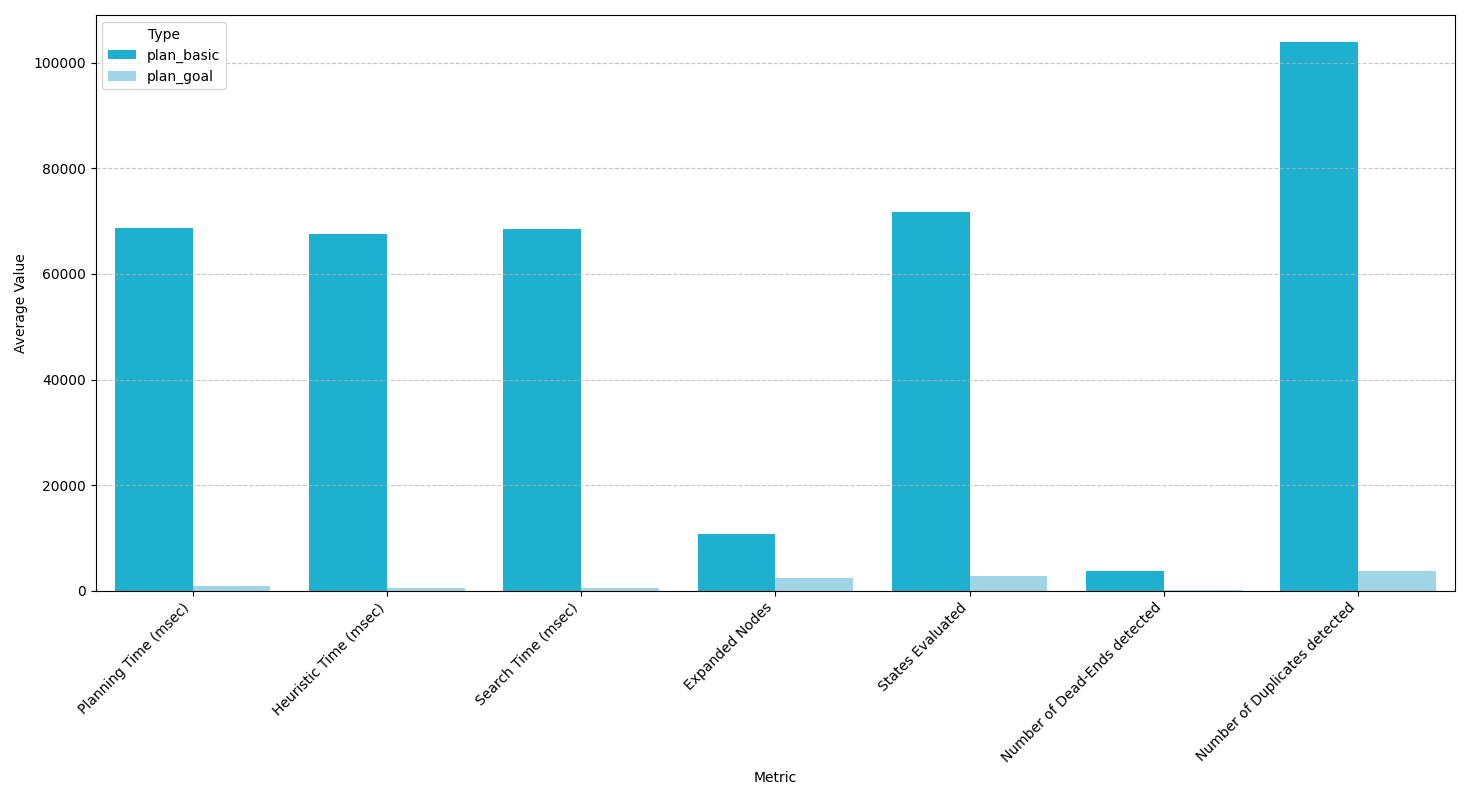
\includegraphics[width=1\textwidth]{/Users/matteo/Documents/Planning-Project/Report/images/basic_goal.png}
    \label{fig:goal}
\end{figure}
\noindent
Dal grafico possiamo evincere una riduzione drastica del numero di \textbf{Stati} e \textbf{Duplicati} valutati,
 che comportano una diminuzione dei tempi di risoluzione, quindi un'ottimizzazione del dominio originale.
\begin{figure}[H]
    \centering
    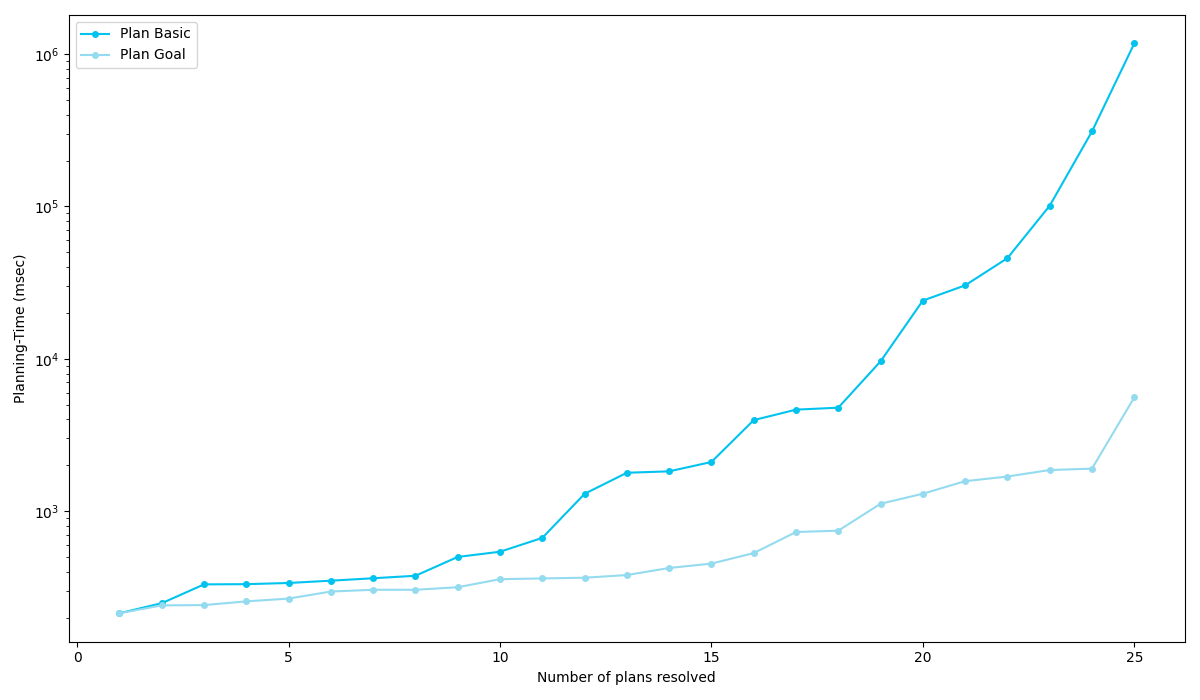
\includegraphics[width=1\textwidth]{/Users/matteo/Documents/Planning-Project/Report/images/time_basic_goal.png}
    \label{fig:goal_states}
\end{figure}
\noindent
Dal seguente grafico\footnote{Non è una comparazione tra i piani degli autori} si può notare come la versione \textbf{Goal} abbia il \textbf{Planning Time}, all'aumentare dei piani risolti, 
un andamento molto più contenuto rispetto alla versione \textbf{Basic}, che ha un andamento esponenziale. Questo è dovuto al fatto che la versione \textbf{Goal} ha un numero di stati e duplicati molto più contenuto.

\section*{Coordinate - version}
La versione \textbf{Coordinate} è stata realizzata con l'obiettivo di ridurre la complessità di inizializzazione della griglia. Nella versione \textbf{Basic} il collegamento tra le varie locatione viene effettuata 
con l'uso del predicato 
\begin{center}
    (next ?from ?to - loc ?d - dir)
\end{center}
comportando quindi, per ogni singola cella della griglia, la definizione di un predicato per ogni direzione.
In questa versione, invece, si è scelto di identificare ogni singola cella della griglia con delle coordinate numeriche, in modo da poter definire le location con una funzione numerica. 
\begin{center}
    (x-coord ?l - location) \hspace{0.5cm} and \hspace{0.5cm} (y-coord ?l - location)
\end{center}
Questa modifica è significativa per la riduzione del numero di predicati,
poichè per problemi definiti su griglie di dimensioni elevate, il numero di predicati cresce in modo esponenziale.\\
Questa versione è un'estensione della versione \textbf{Goal}, in quanto mantiene le modifiche precedenti.
In riferimento a questa versione, dei 46 problemi proposti, ben 30 hanno dato una soluzione. Nel dettaglio abbiamo che :
\begin{table}[H]
    \centering
    \begin{tabular}{|c|c|c|}
        \hline
        \textbf{Domain} & \textbf{Problems} & \textbf{Solved}\\
        \hline
        1 & 33 & 28 \\
        \hline
        2 & 13 & 2\\
        \hline
    \end{tabular}
\end{table}
\noindent
In media è stato riportato un \textbf{Grounding Time} per la versione \textbf{Goal} di \textbf{113,93 msec} e per la versione \textbf{Coordinate} di ben \textbf{3170,13 msec}, un valore molto importante da valutare.
Mentre la lunghezza del piano non ha subito variazioni significative
\begin{figure}[H]
    \centering
    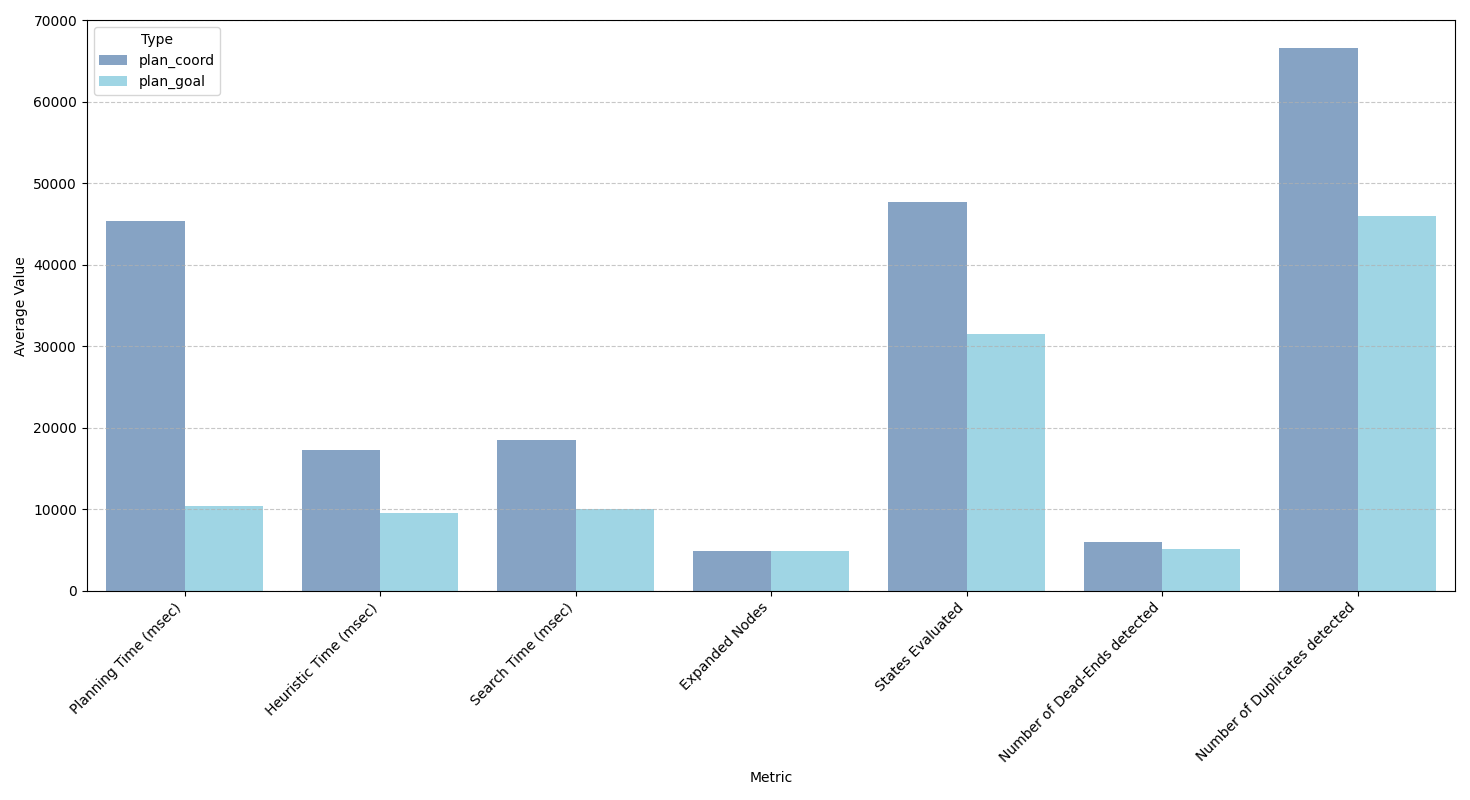
\includegraphics[width=1\textwidth]{/Users/matteo/Documents/Planning-Project/Report/images/goal_coord.png}
    \label{fig:coord}
\end{figure}
\noindent
Dal grafico possiamo notare un incremento,in generale, dei tempi.
Il dato più significativo sta nella disparità dei differenti \textbf{Planning Time}. Nel dettaglio abbiamo, in media, per la versione \textbf{Goal} un tempo meglio di \textbf{4474,25 msec}, contro i \textbf{46574,40 msec} della versione \textbf{Coordinate}, riportando valori \textbf{10} volte maggiori.
\begin{figure}[H]
    \centering
    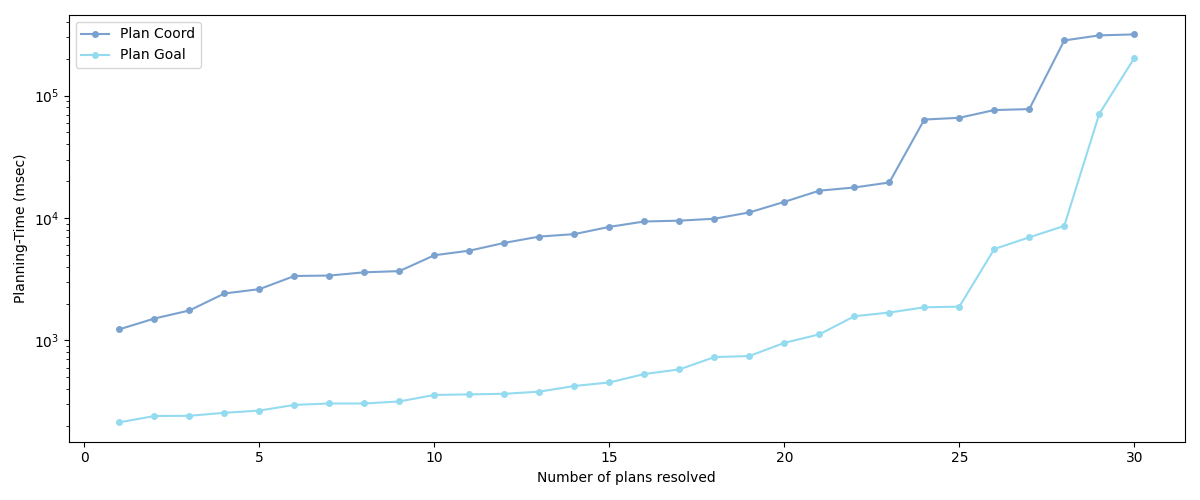
\includegraphics[width=1\textwidth]{/Users/matteo/Documents/Planning-Project/Report/images/time_goal_coord.png}
    \label{fig:coord_states}
\end{figure}
\noindent
Il seguente grafico evidenzia la differenza tra il \textbf{Planning Time} delle due versioni evidenziando la differenza tra i tempi e il loro andamento.

\section*{Count\_ball - version}
La versione \textbf{Count\_ball} è stata realizzata con l'obiettivo di tenere traccia del numero di palle di neve in ogni location, con il secondo fine di evitare la verifica di soddisfacibilità dell'obiettivo.
Per come è strutturato il dominio, se tre palle di neve si trovano in una sola location, esse saranno ordinate in senso decrescente, dal basso verso l'alto, predisposte per la realizzazione di un pupazzo di neve.
Con l'introduzione della funzione 
\begin{center}
    (ball\_count ?l - loc)
\end{center}
evitiamo verifiche superflue, riducendo i tempi di risoluzione. 
Questa versione è un'estensione della versione \textbf{Goal}, in quanto mantiene le modifiche precedenti.
In riferimento a questa versione, dei 46 problemi proposti in 25 hanno dato una soluzione
\begin{table}[H]
    \centering
    \begin{tabular}{|c|c|c|}
        \hline
        \textbf{Domain} & \textbf{Problems} & \textbf{Solved}\\
        \hline
        1 & 33 & 22 \\
        \hline
        2 & 13 & 3\\
        \hline
    \end{tabular}
\end{table}
\noindent
Rispetto la verione \textbf{Goal} si è riportato una riduzione del \textbf{Grounding Time}, rispettivamente per la versione \textbf{Goal} di \textbf{105,17 msec} e per la versione \textbf{Count\_ball} di \textbf{79,25 msec}. 
Inoltre è stato riportato un incremento del \textbf{Plan-Length}, in media di abbiamo che per la versione \textbf{Goal} un valore di \textbf{52 steps} e per la versione \textbf{Count\_ball} di \textbf{66 steps}.
\begin{figure}[H]
    \centering
    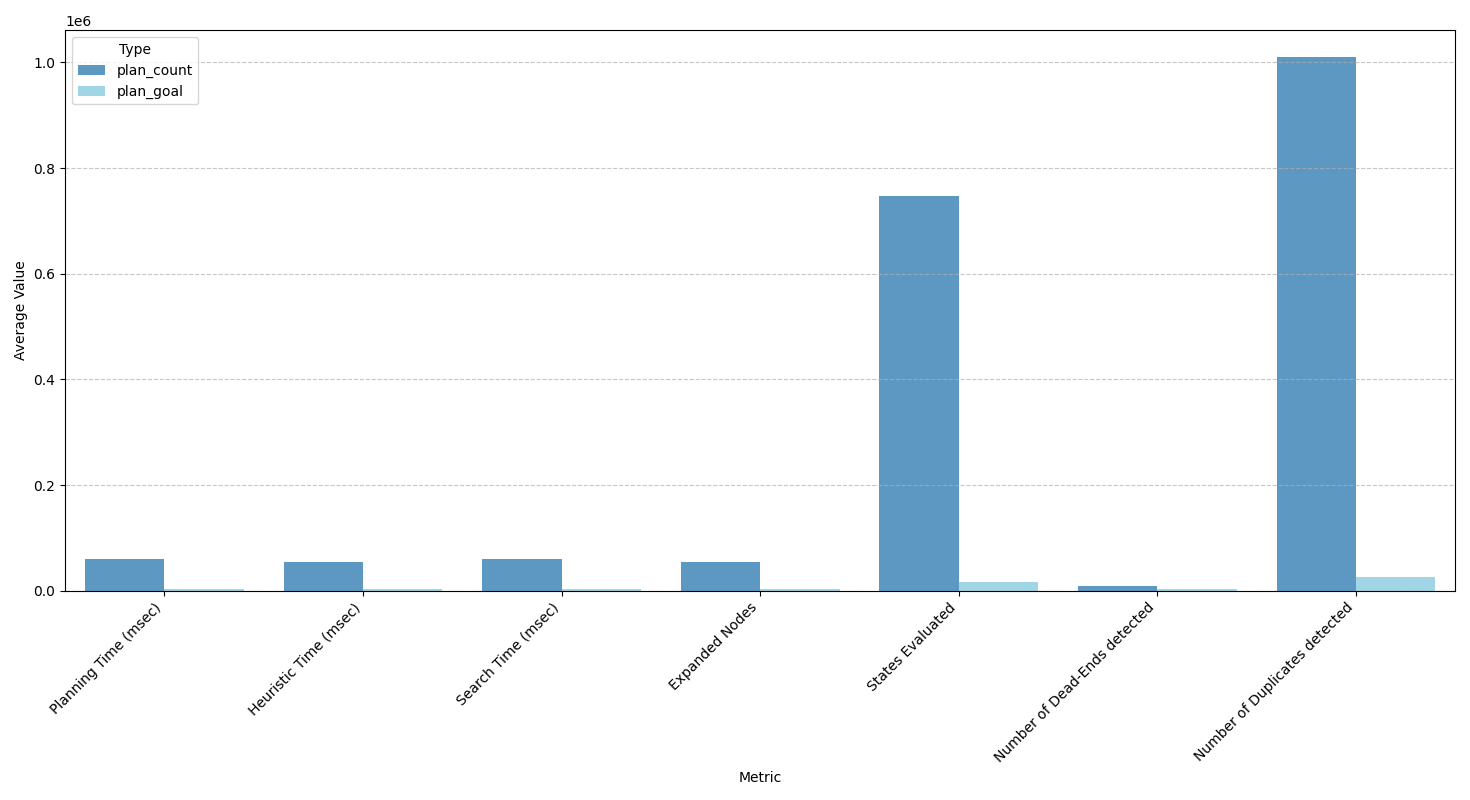
\includegraphics[width=1\textwidth]{/Users/matteo/Documents/Planning-Project/Report/images/goal_count.png}
    \label{fig:count_ball}
\end{figure}
\noindent
Dal seguente grafico possiamo evidenziare la disparità di \textbf{States Evaluated} e \textbf{Duplicated States Evaluated} tra le due versioni. Nel dettaglio abbiamo che:
\begin{table}[H]
    \centering
    \begin{tabular}{|c|c|c|c|}
        \hline
        \textbf{Version} & \textbf{States Evaluated} & \textbf{Duplicated States Evaluated} \\
        \hline
        Goal & 16.561 & 748.227 \\
        \hline
        Count\_ball & 25.266 & 1.010.668 \\
        \hline
    \end{tabular}
\end{table}
\begin{figure}[H]
    \centering
    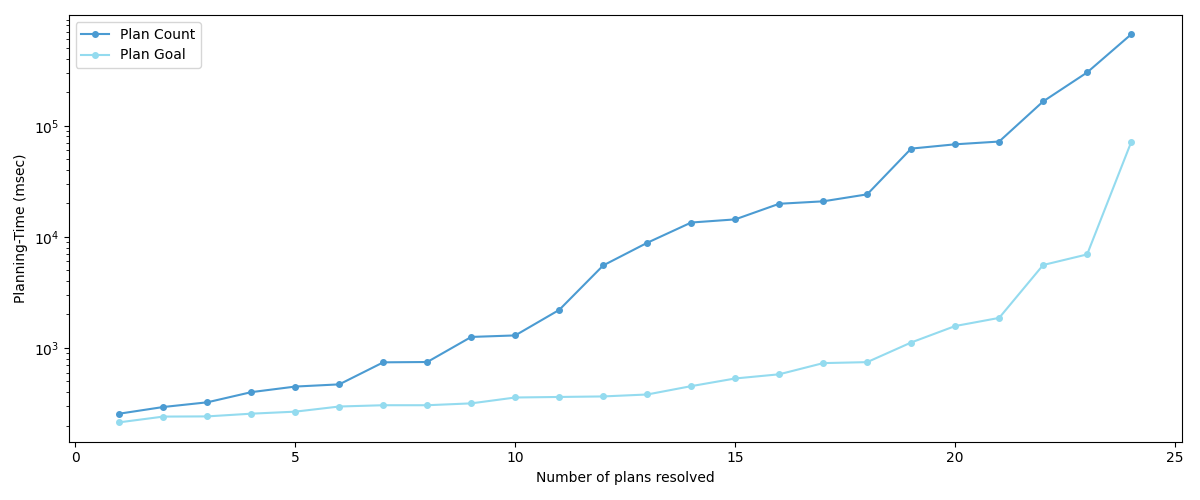
\includegraphics[width=1\textwidth]{/Users/matteo/Documents/Planning-Project/Report/images/time_goal_count.png}
    \label{fig:count_ball_states}
\end{figure}
\noindent
Il seguente grafico evidenzia l'andamento del \textbf{Planning Time} per le due versioni, evidenziando un andamento più contenuto per la versione \textbf{Goal} 
rispetto alla versione \textbf{Count\_ball} che al contrario presenta dei tempi più alti già ad un numero di livelli relativamente basso.

\section*{Analisi generale}     
In generale, l'uso di PDDL Numeric ha portato a dei risultati molto soddisfacenti, in quanto si è ottenuto un incremento del numero di problemi risolti e una riduzione dei tempi di risoluzione.
In particolare, la versione Goal ha riportato un incremento del numero di problemi risolti rispetto alla versione originale, mentre le sue estensioni, ovvero la Coordinate e la Count\_ball hanno risportato dei 
lati negativi che purtroppo non li rendono preferibili rispetto alla versione Goal.\\
Dalla versione Basic alla versione Goal sono stati risolti 9 problemi in più e dal grafico successivo, evidenziamo i tempi ridotti rispetto le altre verisoni.
\begin{figure}[H]
    \centering
    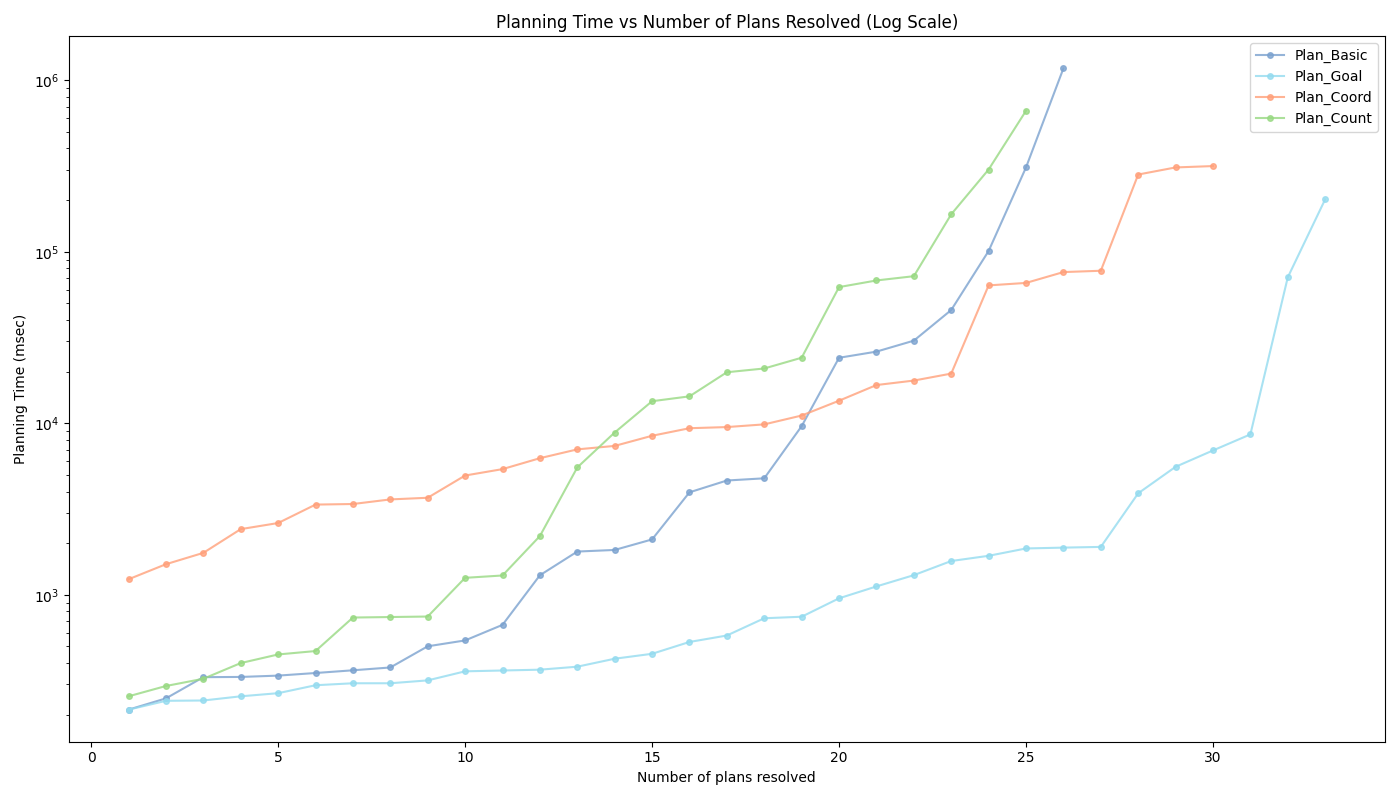
\includegraphics[width=1\textwidth]{/Users/matteo/Documents/Planning-Project/Report/images/all_time.png}
    \label{fig:all_versions}
\end{figure}
La seguente tabella riassume il numero di problemi risolti per ogni versione:
\begin{table}[H]
    \centering
    \begin{tabular}{|c|c|c|c|}
        \hline
        \textbf{Version} & \textbf{Problem 1 and 2} & \textbf{Solved} \\
        \hline
        Basic & 33 - 13 & 25 - 1 \\
        \hline
        Goal & 33 - 13& 31 - 2  \\
        \hline
        Coordinate & 33 - 13 & 28 - 2 \\
        \hline
        Count\_ball & 33 - 13 & 22 - 3 \\
        \hline
    \end{tabular}
\end{table}
\vspace{1cm}
In definitiva, ogni versione evidenzia delle caratteristiche significative :
\begin{itemize}
    \item \textbf{Basic} con piani particolarmente lunghi e un numero di duplicati relativamente alto;
    \item \textbf{Goal} ha una pianificazione molto veloce con pochi nodi espansi e duplicati, ma poco adatto a scenari complessi;
    \item \textbf{Coordinate} è equilibrato, ha un piano medio-lungo riuscendo a mantenere sotto controllo i duplicati, con tempi di pianificazione moderati;
    \item \textbf{Count\_ball} è adatto a piani articolati, ma ha un altissimo umero di duplicati e tempi lunghi; 
\end{itemize}





























\end{document}
